\documentclass[notheorems,envcountsect,pdfpagemode=FullScreen,12pt]{beamer}
\usepackage{amssymb}
\usepackage{amsmath}
\usepackage{color}
\usepackage{graphicx}
\usepackage{float}
\usepackage[all,cmtip]{xy}
\usepackage{enumerate}
\usefonttheme[onlymath]{serif}
\usetheme{Boadilla}
\usecolortheme{beaver}

\usepackage{algorithm}
\usepackage{algorithmicx}
\usepackage{algpseudocode}
\algnewcommand\algorithmicinput{\textbf{Input:}}
\algnewcommand\Input{\item[\algorithmicinput]}
\algnewcommand\algorithmicoutput{\textbf{Output:}}
\algnewcommand\Output{\item[\algorithmicoutput]}

\makeatletter
\newenvironment{breakablealgorithm}
  {% \begin{breakablealgorithm}
   \begin{center}
     \refstepcounter{algorithm}% New algorithm
     \hrule height.8pt depth0pt \kern2pt% \@fs@pre for \@fs@ruled
     \renewcommand{\caption}[2][\relax]{% Make a new \caption
       {\raggedright\textbf{\ALG@name~\thealgorithm} ##2\par}%
       \ifx\relax##1\relax % #1 is \relax
         \addcontentsline{loa}{algorithm}{\protect\numberline{\thealgorithm}##2}%
       \else % #1 is not \relax
         \addcontentsline{loa}{algorithm}{\protect\numberline{\thealgorithm}##1}%
       \fi
       \kern2pt\hrule\kern2pt
     }
  }{% \end{breakablealgorithm}
     \kern2pt\hrule\relax% \@fs@post for \@fs@ruled
   \end{center}
  }
\makeatother

\usepackage{tikz-cd}
\usetikzlibrary{cd}

\usepackage{amsthm}
\setbeamertemplate{theorem}[amsstyle]
\setbeamertemplate{theorems}[numbered]
\theoremstyle{plain}
\newtheorem{theo}{Theorem}
\newtheorem{lem}{Lemma}

\theoremstyle{definition}
\newtheorem{defin}{Definition}

\theoremstyle{example}
\newtheorem{example}{Example}

\title{Algorithms for Matrix Manifold Optimization}
\author[Zihan Zhou]{Student: Zihan Zhou\texorpdfstring{\\ Advisor: Enbin Song}{}}
\institute[Sichuan University]{{\large Sichuan University}}
\date{May, 28, 2020}

\begin{document}

\begin{frame}
\maketitle
\begin{figure}[ht]
\centering

\includegraphics[height=2cm]{sculogo.png}
\end{figure}
\end{frame}

\begin{frame}
\frametitle{Introduction}
\begin{itemize}
\item A preliminary introduction to \textcolor{red}{manifold optimization}, i.e.
$\min\limits_{x\in\mathcal{M}}f(x)$, where $\mathcal{M}$ is a Riemannian manifold.
\item Numerical implementation of \textcolor{blue}{line-search method} and \textcolor{blue}{Riemannian BFGS method}.
\end{itemize}
\end{frame}

\begin{frame}
\frametitle{First-Order Geometry}
\quad In these slides, all manifolds $\mathcal{M}$ are assumed to be Riemannian, and all functions are assumed to be smooth.\par
\quad We use the notation $g_x(\xi_x,\zeta_x)=\langle\xi_x,\zeta_x\rangle_x$ to denote the \textcolor{blue}{inner product} of two elements $\xi_x$ and $\zeta_x$ of $T_x\mathcal{M}$.
\\~\\
\begin{defin}[Riemannian gradient]
Given a smooth scalar field $f$ on a Riemannian manifold $\mathcal{M}$, the \textcolor{red}{Riemannian gradient} of $f$ at $x$, denoted by $\mathrm{grad}f(x)$, is the unique element of $T_x\mathcal{M}$ that satisfies
$$\langle\mathrm{grad}f(x),\xi\rangle_x=\mathrm{D}f(x)[\xi], \forall \xi\in T_x\mathcal{M}.$$
\end{defin}
\end{frame}

\begin{frame}
\frametitle{Embedded Submanifold}
\quad We call a manifold $\mathcal{N}$ an \textcolor{red}{embedded submanifold} of manifold $\mathcal{M}$ if $\mathcal{N}\subset\mathcal{M}$ and there exists an embedded mapping $F:\mathcal{N}\to\mathcal{M}$.
\\~\\
\begin{example}[Sphere]
$S^n:=\{x\in\mathbb{R}^{n+1}:x^Tx=1\}$ is an embedded submanifold of $\mathbb{R}^{n+1}$.
\end{example}
\begin{example}[Stiefel manifold]
$\mathrm{St}(p,n):=\{X\in\mathbb{R}^{n\times p}:X^TX=I_p\}$ is an embedded submanifold of $\mathbb{R}^{n\times p}$. 
\end{example}
\end{frame}

\begin{frame}
\frametitle{Embedded Submanifold}
\quad If $\mathcal{M}$ is an embedded submanifold of $\mathbb{R}^n$, the tangent space of arbitrary $x\in\mathcal{M}$ is an affine subspace of $\mathbb{R}^n$.
\\~\\
\quad Let $\mathrm{P}_x$ and $\mathrm{P}^\perp_x$ denote the \textcolor{red}{projection} onto $T_x\mathcal{M}$ and its orthocomplement, respectively.
\\~\\
\quad $\mathrm{grad}f|_{\mathcal{M}}(x)=\mathrm{P}_x\mathrm{grad}f(x)$.
\end{frame}

\begin{frame}
\frametitle{Quotient Manifold}
\quad Let $\mathcal{M}$ be a manifold equipped with an equivalence relation $\sim$, and define the natural projection $\pi:\mathcal{M}\to\mathcal{M}/\sim$ by $x\mapsto[x]$.\par
\quad We call $\mathcal{M}/\sim$ a \textcolor{red}{quotient manifold} of $\mathcal{M}$ if $\mathcal{M}/\sim$ is a manifold and $\pi$ is a submersion.
\\~\\
\begin{example}[Grassmann manifold]
$\mathrm{Grass}(p,n)\simeq\mathbb{R}^{n\times p}_*/\mathrm{GL}_p$ is a quotient manifold of $\mathbb{R}^{n\times p}_*$, where $\mathbb{R}^{n\times p}_*$ is the set of all $n\times p$ matrices with full column rank.
\end{example}
\end{frame}

\begin{frame}
\frametitle{Quotient Manifold}
\quad If $\mathcal{M}=\overline{\mathcal{M}}/\sim$ is a quotient manifold of $\overline{\mathcal{M}}$, the equivalence class $\pi^{-1}(x)$ is an embedded submanifold of $\overline{\mathcal{M}}$, where $x\in\mathcal{M}$.
\\~\\
\quad Hence $\pi^{-1}(x)$ admits a tangent space $\mathcal{V}_{\overline{x}}=T_{\overline{x}}(\pi^{-1}(x))$ called the \textcolor{red}{vertical space} at $\overline{x}$.
\\~\\
\quad A mapping $\mathcal{H}$ that assigns to each element $\overline{x}$ of $\overline{\mathcal{M}}$ a subspace $\mathcal{H}_{\overline{x}}$ of $T_{\overline{x}}\overline{\mathcal{M}}$ complementary to $\mathcal{V}_{\overline{x}}$ is called a \textcolor{red}{horizontal distribution} on $\overline{\mathcal{M}}$.
\\~\\
\quad If $\overline{\mathcal{M}}$ endowed with a horizontal distribution, there exists unique vector $\overline{\xi}_{\overline{x}}\in\mathcal{H}_{\overline{x}}$ satisfies $\mathrm{D}\pi(\overline{x})[\overline{\xi}_{\overline{x}}]=\xi$. The vector $\overline{\xi}_{\overline{x}}$ is called the \textcolor{red}{horizontal lift} of $\xi$ at $\overline{x}$.
\end{frame}

\begin{frame}
\frametitle{Quotient Manifold}
\quad We use the notation $\mathrm{P}^h_{\overline{x}}\xi_{\overline{x}}$ and $\mathrm{P}^v_{\overline{x}}\xi_{\overline{x}}$ for the \textcolor{red}{projection} of $\xi_{\overline{x}}\in T_{\overline{x}}\overline{\mathcal{M}}$ onto $\mathcal{H}_{\overline{x}}$ and $\mathcal{V}_{\overline{x}}$.
\\~\\
\quad $g_x(\xi_x,\eta_x):=\overline{g}_{\overline{x}}(\overline{\xi}_{\overline{x}},\overline{\eta}_{\overline{x}},\overline{\eta}_{\overline{x}})$.
\\~\\
\quad $\overline{\mathrm{grad}f_{\overline{x}}}=\mathrm{grad}\overline{f}(\overline{x})$.
\end{frame}

\begin{frame}
\frametitle{Retraction}
\begin{defin}[Retraction]
A \textcolor{red}{retraction} on a manifold $\mathcal{M}$ is a smooth mapping $R:T\mathcal{M}\to\mathcal{M}$ with the following properties. Let $R_x$ denote the restriction of $R$ to $T_x\mathcal{M}$.
\begin{itemize}
\item[(i)] $R_x(0_x)=x$;
\item[(ii)] $\mathrm{D}R_x(0_x)=\mathrm{id}_{T_x\mathcal{M}}$.
\end{itemize}
\end{defin}
\end{frame}

\begin{frame}
\frametitle{Sphere}
cost function: $f(x)=x^TAx, x\in S^n$
\\~\\
metric: $\langle\xi,\eta\rangle=\xi^T\eta$
\\~\\
tangent space: $T_xS^n=\{\xi\in\mathrm{R}^{n+1}:x^T\xi=0\}$
\\~\\
projection onto tangent space: $\mathrm{P}_x\xi=(I-xx^T)\xi$
\\~\\
retraction: $R_x(\xi)=\mathrm{qf}(x+\xi)$
\end{frame}

\begin{frame}
\frametitle{Stiefel manifold}
cost function: $f(x)=X^TAX, X^TX=I_p$
\\~\\
metric: $\langle Z_1,Z_2\rangle=\mathrm{tr}(Z_1^T Z_2)$
\\~\\
tangent space: $T_x\mathrm{St}(n,p)=\{Z\in\mathrm{R}^{n\times p}:\mathrm{sym}(X^T Z)=0\}$
\\~\\
projection onto tangent space: $\mathrm{P}_X Z=Z-X\mathrm{sym}(X^TZ)$
\\~\\
retraction: $R_X(Z)=\mathrm{qf}(X+Z)$
\end{frame}

\begin{frame}
\frametitle{Grassmann manifold}
cost function: $\mathrm{span}(Y)\mapsto\overline{f}(Y)=\mathrm{tr}((Y^TY)^{-1}Y^TAY)$
\\~\\
metric: $\langle\xi,\eta\rangle_{\mathrm{span}(Y)}=\mathrm{tr}((Y^TY)^{-1}Z_1^TZ_2)$
\\~\\
horizontal space: $\mathcal{H}_Y=\{Z\in\mathrm{R}^{n\times p}:Y^T Z=0\}$
\\~\\
projection onto horizontal space: $\mathrm{P}_Y^h Z=Z-Y(Y^TY)^{-1}Y^TZ$
\\~\\
retraction: $R_{\mathrm{span}(Y)}(\xi)=\mathrm{span}(Y+\overline{\xi}_Y)$
\end{frame}

\begin{frame}
\frametitle{First-Order Algorithms}
\begin{algorithm}[H]
\caption{Armijo line search for the Rayleigh quotient on manifold}
\begin{algorithmic}[1]
\Require Retraction $R$; symmetric matrix A; scalars $\overline{\alpha}$, $\beta$, $\sigma\in(0,1)$.
\Input Initial iterate $x_0\in\mathcal{M}$.
\Output Sequence of iterates $\{x_k\}$.
\For{$k=0,\ 1,\ 2,\dots$}
\State Compute $\eta_k=-\mathrm{grad}f(x_k)$.
\State Find the smallest integer $m\geqslant 0$ such that
$$f(R_{x_k}(\overline{\alpha}\beta^m\eta_k))\leqslant f(x_k)-\sigma\overline{\alpha}\beta^m g_{x_k}(\eta_k,\eta_k),$$
\quad\ \,where $t_k^A$ is the Armijo step size for the given $\overline{\alpha}, \beta, \sigma, \eta_k$.
\State Set $x_{k+1}=R_{x_k}(\overline{\alpha}\beta^m\eta_k)$.
\EndFor
\end{algorithmic}
\end{algorithm}
\end{frame}

\begin{frame}
\frametitle{Second-Order Geometry}
\quad Let $\nabla$ denote the Leci-Civita connection of $\mathcal{M}$, then we can define the \textcolor{red}{Riemannian Hessian} by $\mathrm{Hess}f(x)[\xi_x]=\nabla_{\xi_x}\mathrm{grad}f$.
\end{frame}

\begin{frame}
\frametitle{Vector Transport}
\begin{defin}[vector transport]
A \textcolor{red}{vector transport} on a manifold $\mathcal{M}$ is a smooth mapping
$$\mathcal{T}:T\mathcal{M}\otimes T\mathcal{M}\to T\mathcal{M}:(\eta_x,\xi_x)\mapsto\mathcal{T}_{\eta_x}(\xi_x)$$
satisfying the following properties.
\begin{itemize}
\item[(i)] $\mathcal{T}_{0_x}\xi_x=\xi_x$;
\item[(ii)] $\mathcal{T}_{\eta_x}(a\xi_x+b\zeta_x)=a\mathcal{T}_{\eta_x}\xi_x+b\mathcal{T}_{\eta_x}\zeta_x$;
\end{itemize}
\end{defin}
\end{frame}

\begin{frame}
\frametitle{Vector Transport}
\begin{defin}[vector transport]
\begin{itemize}
\item[(iii)] Exists a retraction $R$, called the retraction associated with $\mathcal{T}$, such that the following diagram commutes
$$\begin{tikzcd}[ampersand replacement=\&]
(\eta_x,\xi_x)\arrow[d] \arrow[r, "\mathcal{T}"] \& \mathcal{T}_{\eta_x}(\xi_x)\arrow[d, "\pi"]\\
\eta_x\arrow[r, "R"swap] \& \pi(\mathcal{T}_{\eta_x}(\xi_x))
\end{tikzcd}$$
where $\pi(\mathcal{T}_{\eta_x}(\xi_x))$ denotes the foot of the tangent vector $\mathcal{T}_{\eta_x}(\xi_x)$.
\end{itemize}
\end{defin}
\end{frame}

\begin{frame}
\frametitle{Vector Transport}
Vector transport on embedded submanifold: $\mathcal{T}_{\eta_x}\xi_x=\mathrm{P}_{R_x(\eta_x)}\xi_x$.
\\~\\
Vector transport on quotient manifold: $\overline{(\mathcal{T}_{\eta_x}\xi_x)}_{\overline{x}+\overline{\eta}_{\overline{x}}}=\mathrm{P}^h_{\overline{x}+\overline{\eta}_{\overline{x}}}\overline{\xi}_{\overline{x}}$.
\end{frame}

\begin{frame}
\footnotesize
\frametitle{Second-Order Algorithms}
\begin{breakablealgorithm}
\caption{Riemannian BFGS method}
\begin{algorithmic}[1]
\Require Vector transport operator $\mathcal{T}$ with associated retraction $R$.
\Input Initial iterate $x_0\in\mathcal{M}$; symmetric positive-definite operator $\mathcal{B}_0:T_{x_0}\mathcal{M}\to T_{x_0}\mathcal{M}$.
\Output Sequence of iterates $\{x_k\}$.
\For{$k=0,\ 1,\ 2,\dots$}
\State Obtain $\xi_k$ by solving $\mathcal{B}_k\xi_k=-\mathrm{grad}f(x_k)$.
\State Set $\eta_k=\alpha_k\xi_k$, where $\alpha_k$ is computed by a line-search procedure.
\State Set $x_{k+1}=R_{x_k}(\alpha_k\xi_k)$.
\State Compute $s_k=\mathcal{T}_{\eta_k}\eta_k$ and $y_k=\mathrm{grad}f(x_{k+1})-\mathcal{T}_{\eta_k}(\mathrm{grad}f(x_k))$.
\State Define the linear operator $\mathcal{B}_{k+1}:T_{x_{k+1}}\mathcal{M}\to T_{X_{k+1}}\mathcal{M}$ by
$$\mathcal{B}_{k+1}\zeta=\tilde{\mathcal{B}}_k\zeta-\frac{\langle s_k,\tilde{\mathcal{B}}_k\zeta\rangle}{\langle s_k,\tilde{\mathcal{B}}_k s_k\rangle}\tilde{\mathcal{B}}_k s_k+\frac{\langle y_k,\zeta\rangle}{\langle y_k,s_k\rangle}\zeta,\ \forall \zeta\in T_{x_{k+1}}\mathcal{M},$$
\quad\ \,where $\tilde{\mathcal{B}}_k=\mathcal{T}_{\eta_k}\circ\mathcal{B}_k\circ(\mathcal{T}_{\eta_k})^{-1}$.
\EndFor
\end{algorithmic}
\end{breakablealgorithm}
\end{frame}

\begin{frame}
\frametitle{Numerical Results}
\begin{figure}[h]
\centering
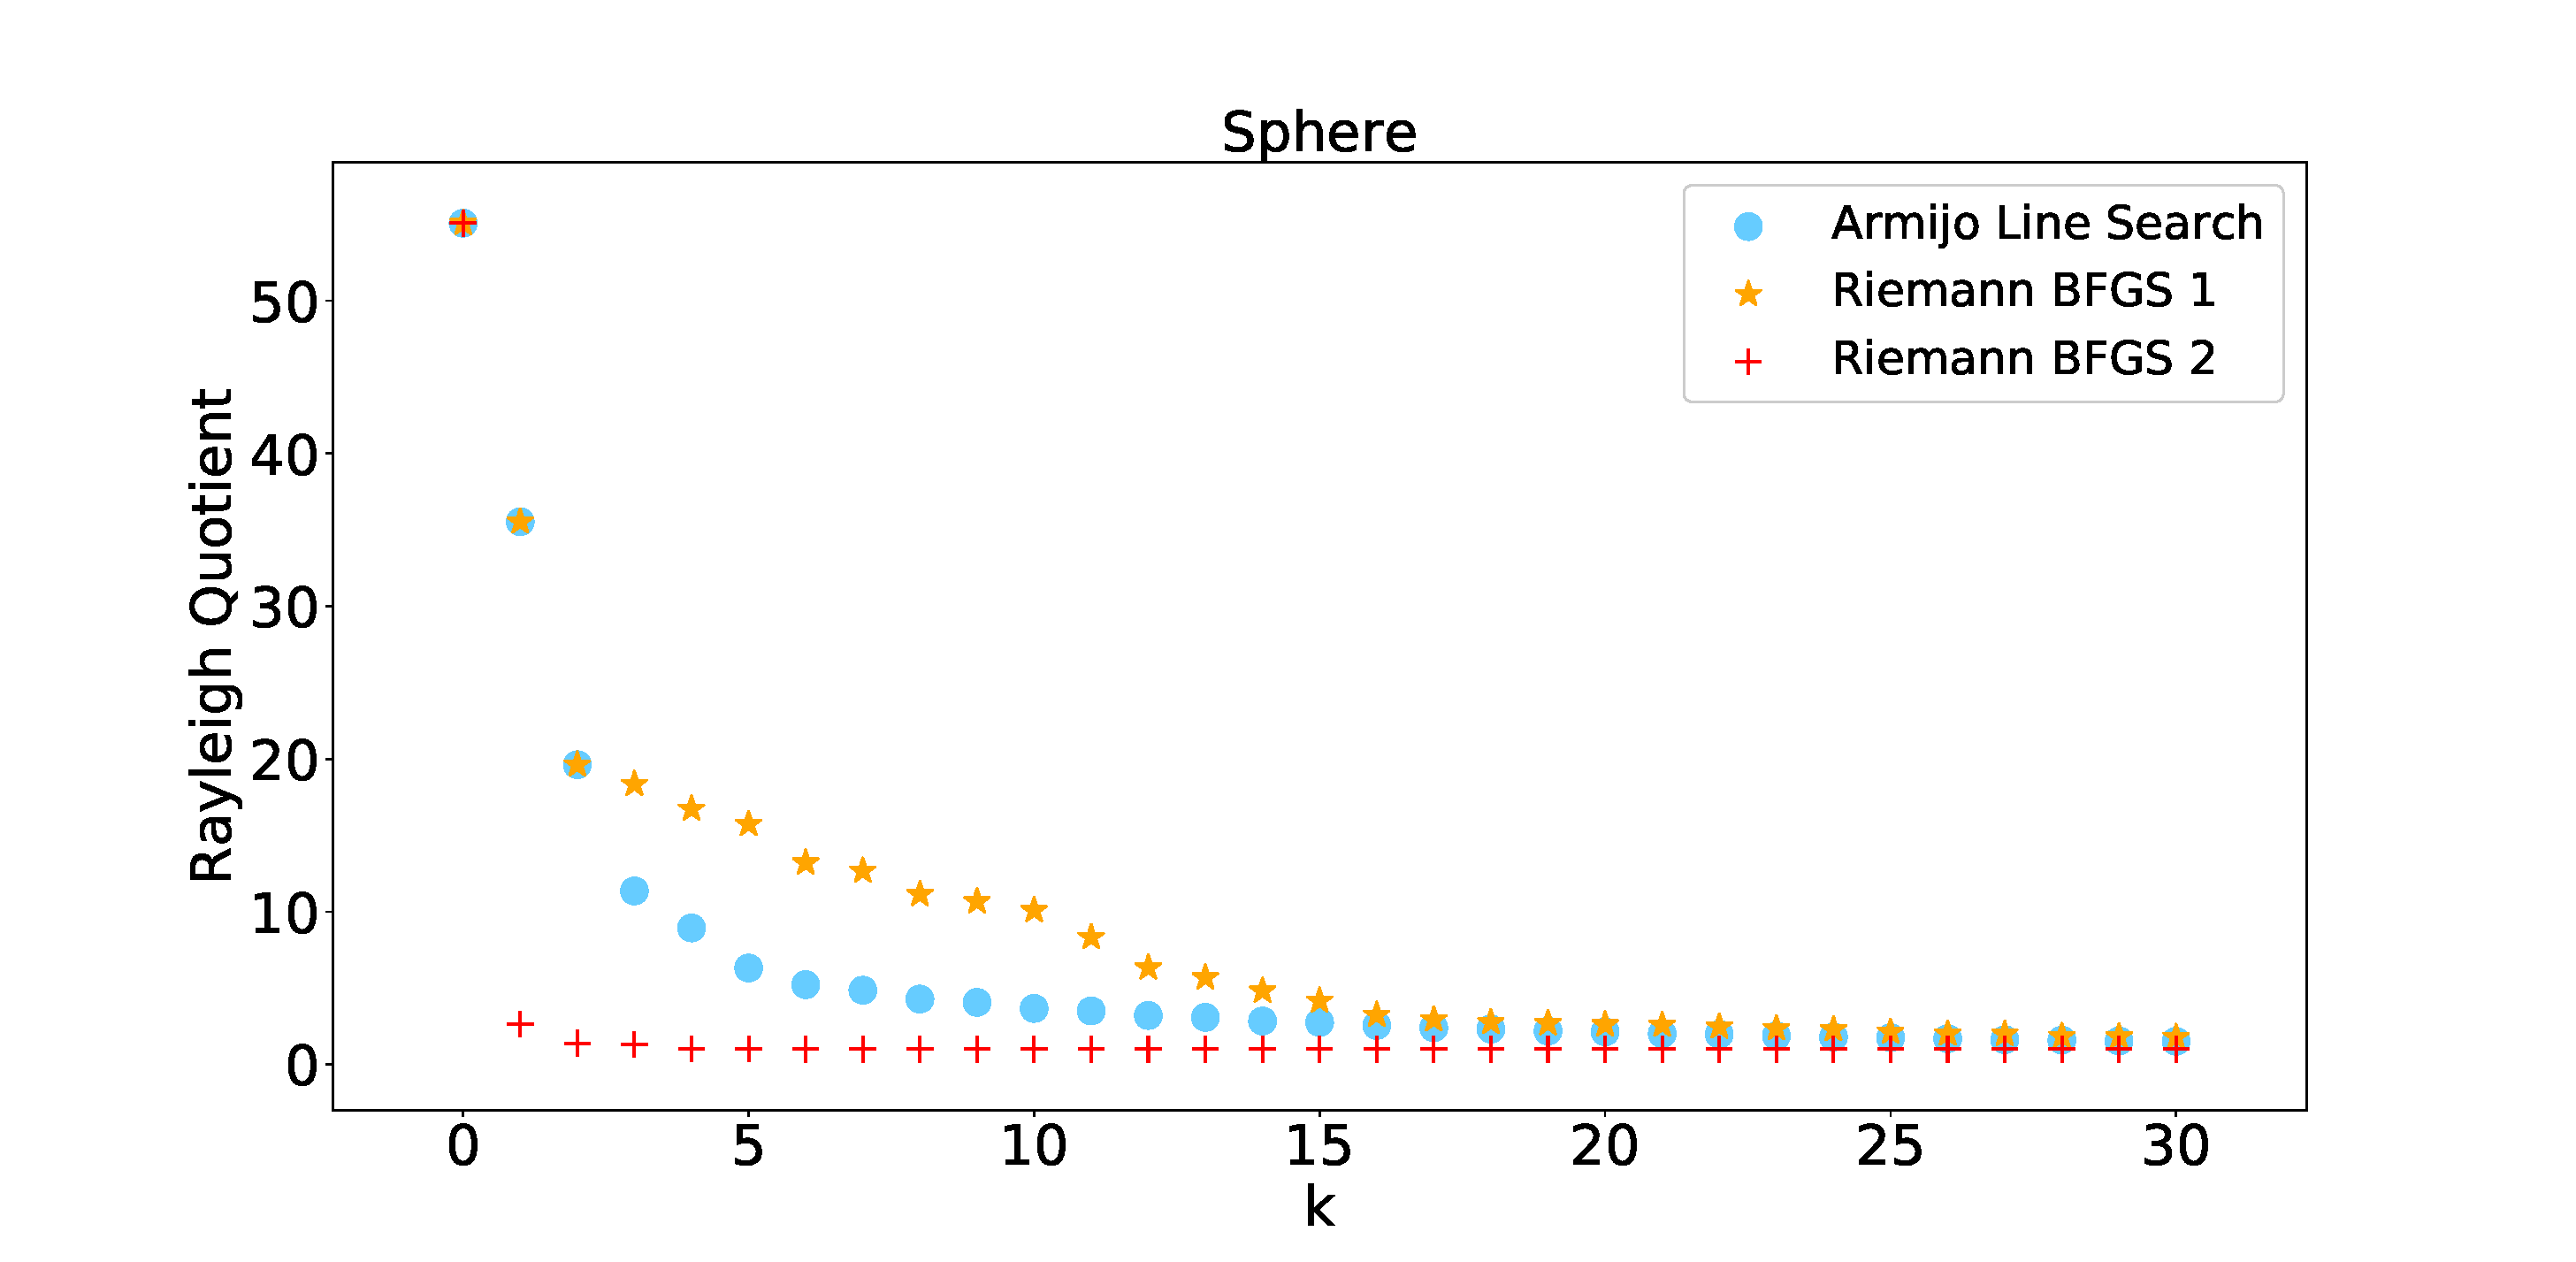
\includegraphics[width=0.8\textwidth]{1.eps}
\caption{\small Minimization of the Rayleigh quotient of $A=\mathrm{diag}(1,2,\dots,100)$ on sphere, with $\overline{\alpha}=1, \beta=\sigma=0.5$.\newline The `Riemann BFGS 1' means that we choose identity mapping as $\mathcal{B}_0$, and $\mathcal{B}_0\xi=A\xi$ for 'Riemann BFGS 2'.}
\end{figure}
\end{frame}

\begin{frame}
\frametitle{Numerical Results}
\begin{figure}[H]
\centering
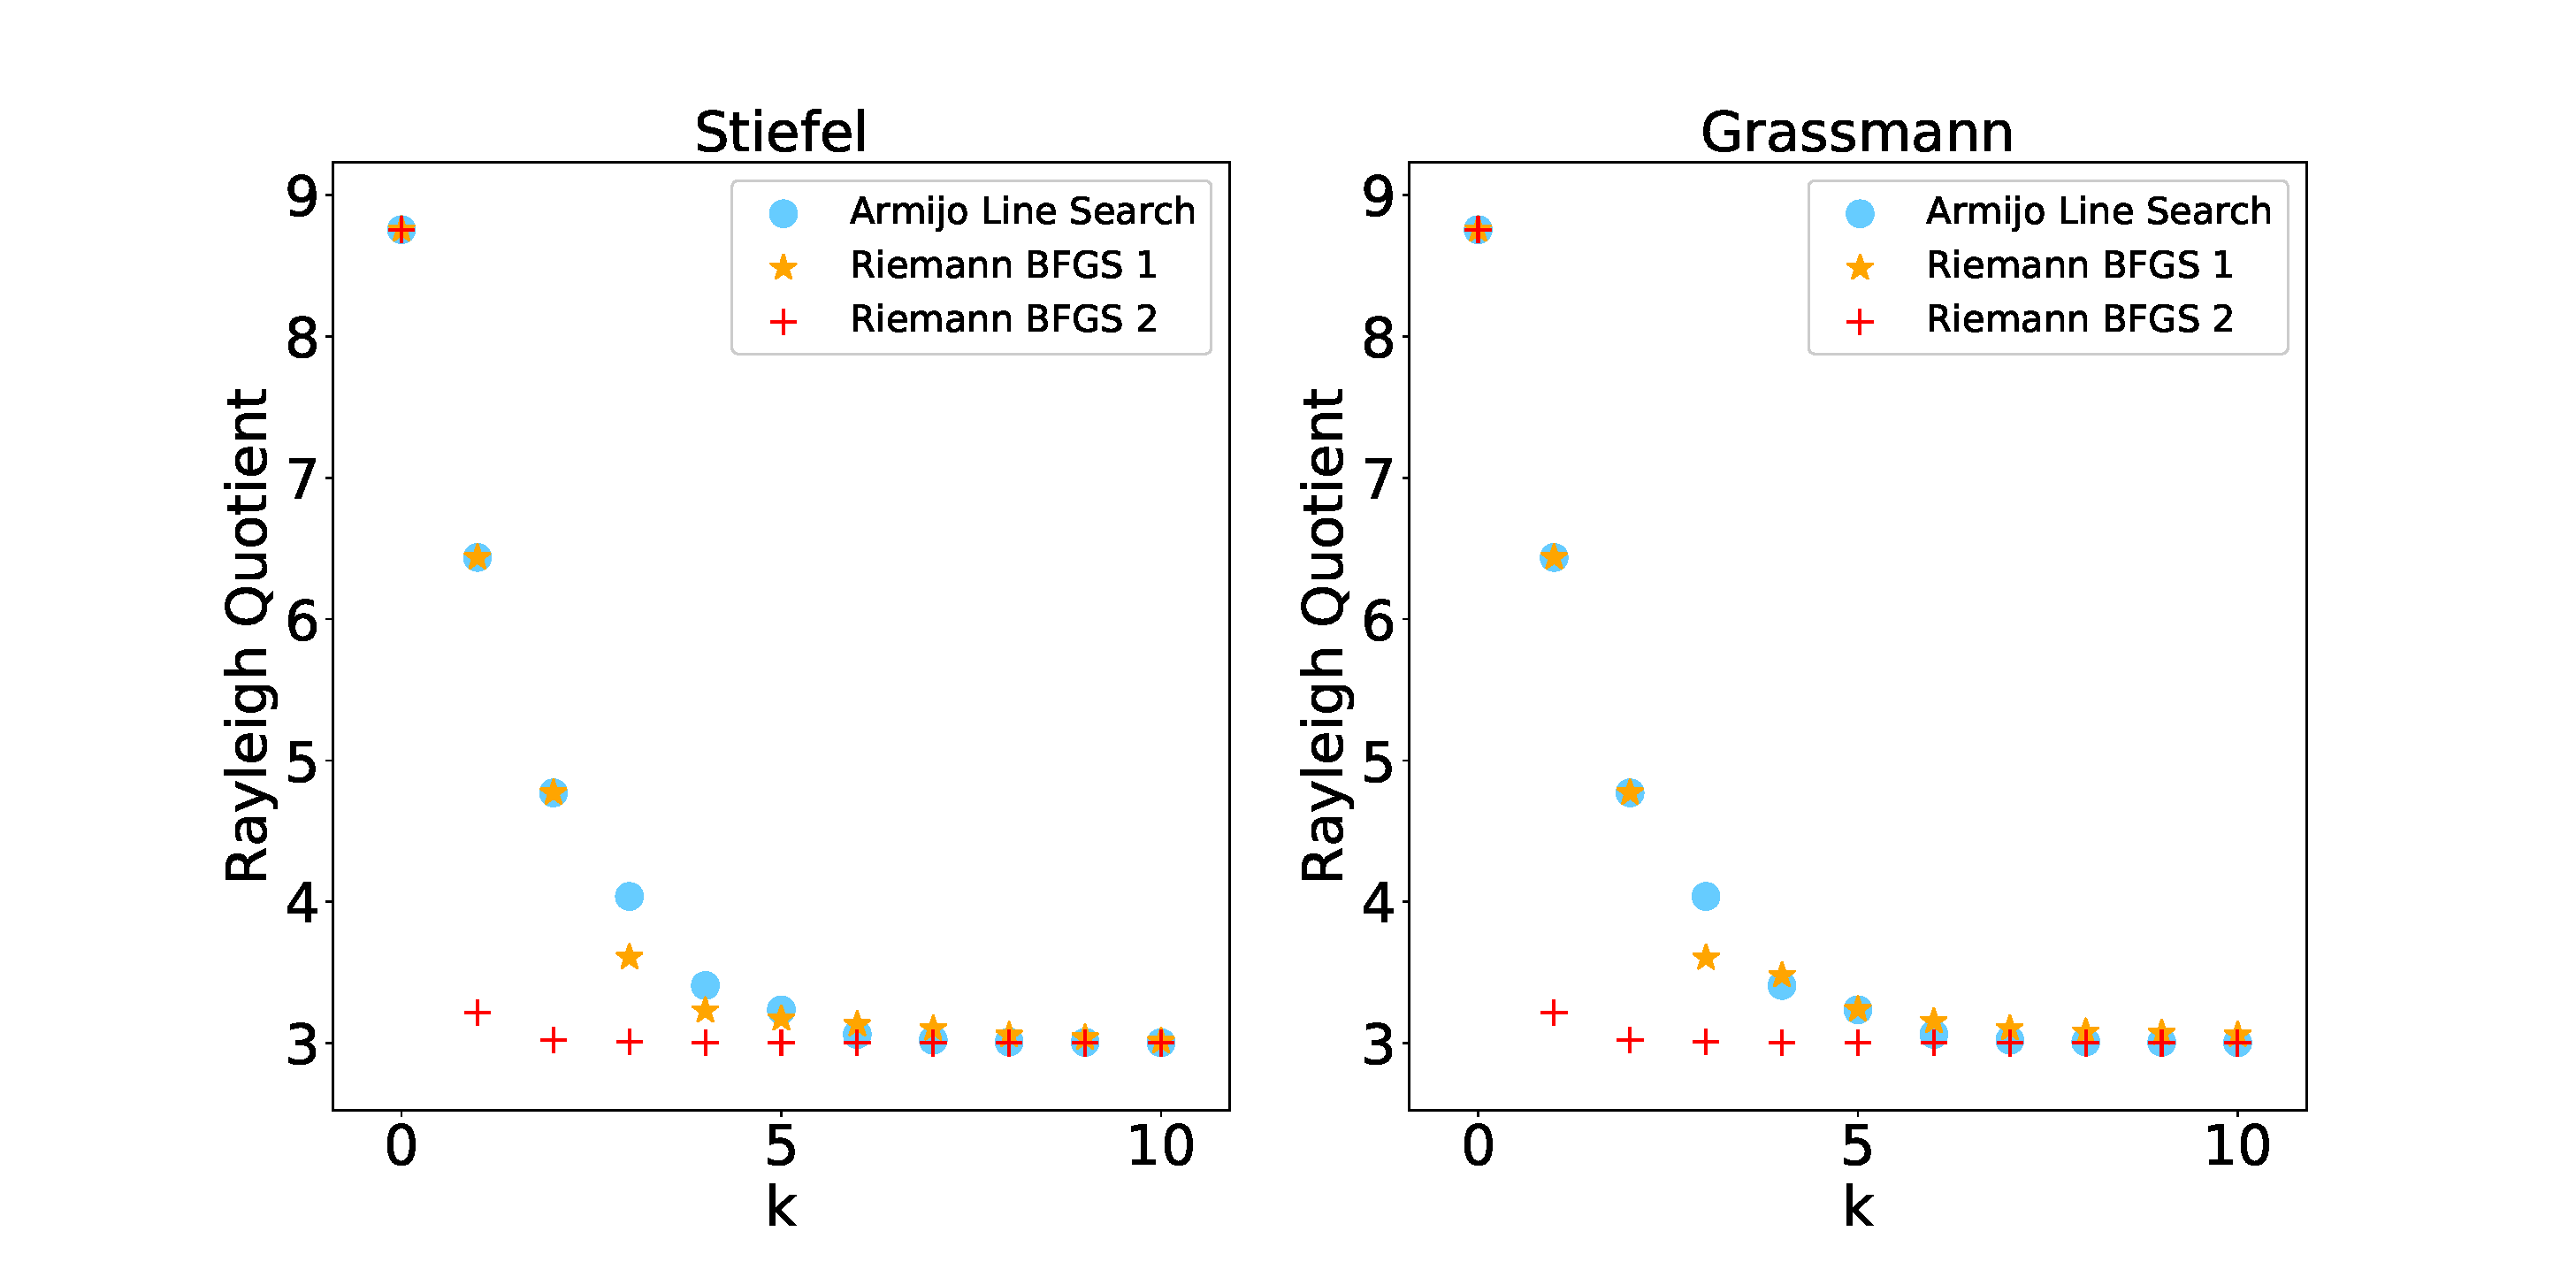
\includegraphics[width=0.8\textwidth, height=120pt]{2.eps}
\caption{Minimization of the Rayleigh quotient of $A=\mathrm{diag}(1,2,\dots,10)$ on Stiefel manifold and Grassmann manifold, with $p=2$, $\overline{\alpha}=1$, $\beta=\sigma=0.5$.\newline The `Riemann BFGS 1' means that we choose identity mapping as $\mathcal{B}_0$, and $\mathcal{B}_0\xi=A\xi$ for 'Riemann BFGS 2'.}
\end{figure}
\end{frame}

\begin{frame}
\frametitle{References}
\begin{thebibliography}{99}
\bibitem{1} Hu, Jiang and Liu, Xin and Wen, Zaiwen and Yuan, Yaxiang. A Brief Introduction to Manifold Optimization. arXiv preprint arXiv:1906.05450, 2019.
\bibitem{2} Absil, P-A and Mahony, Robert and Sepulchre, Rodolphe. Optimization algorithms on matrix manifolds. Princeton University Press, 2009.
\bibitem{3} Horn, Roger A and Johnson, Charles R. Matrix analysis. Cambridge university press, 2012.
\bibitem{4} Chang, Kung-Ching. Methods in nonlinear analysis. Springer Science \& Business Media, 2006.
\end{thebibliography}
\end{frame}

\begin{frame}
\frametitle{References}
\begin{thebibliography}{99}
\bibitem{5} Absil, P-A and Mahony, Robert and Sepulchre, Rodolphe. Riemannian geometry of Grassmann manifolds with a view on algorithmic computation, volume 80. Acta Applicandae Mathematica, 2004.
\bibitem{6} O'neill, Barrett. Semi-Riemannian geometry with applications to relativity. Academic press, 1983.
\bibitem{7} Huang, Wen and Absil, P-A and Gallivan, Kyle A. A Riemannian BFGS method without differentiated retraction for nonconvex optimization problems, volume 28. SIAM Journal on Optimization, 2018.
\bibitem{8} Kobayashi, Shoshichi and Nomizu, Katsumi. Foundations of differential geometry. 1963.
\end{thebibliography}
\end{frame}

\begin{frame}	
\center{\huge Thank you!}
\end{frame}
\end{document}